\documentclass[12pt,a4paper]{article}
\usepackage[width=.75\textwidth]{caption}
\usepackage{graphicx}
\usepackage{authblk}
\usepackage{amsmath}
\usepackage{amsfonts}
\usepackage{braket}
\usepackage{epigraph}
%\usepackage{mathrsfs}
\usepackage[mathscr]{euscript}
\usepackage[top=2cm, bottom=2cm, left=2cm, right=2cm]{geometry}
\usepackage{fancyhdr}
\newcommand{\dv}[1]{\mathrm{d} #1 \text{ }}
\newcommand*\diff{\mathop{}\!\mathrm{d}}
\newcommand\restr[2]{{% we make the whole thing an ordinary symbol
  \left.\kern-\nulldelimiterspace % automatically resize the bar with \right
  #1 % the function
  \vphantom{\big|} % pretend it's a little taller at normal size
  \right|_{#2} % this is the delimiter
  }}
\setlength{\epigraphwidth}{0.8\textwidth}

% \pagestyle{fancy}
\begin{document}

%title and author details
\title{Localization of the Unruh Effect}
\author[1]{Kevin Player\footnote{kjplaye@gmail.com}}

\maketitle

\epigraph{The Unruh effect tells us that what we call particles is really just a matter of perspective.}{Lee Smolin}


\abstract{We present a framework that interpolates between the standard thermal interpretation of the Unruh effect and a fully localized, non-thermal excitation. In a uniformly accelerating frame, the extended support of Rindler modes across the wedge leads to red- and blue-shifts, mixing frequencies in a way that gives rise to the familiar thermal response. To refine this picture, we introduce a partially localized perspective: by employing modular automorphisms, we map modes between nested Rindler wedges and analyze their localization properties. We further interpolate to compactly supported wave packets using parabolic cylinder functions, enabling a smooth transition from global to local behavior. Rather than attributing particle detection to the horizons thermality, this construction reframes the effect as the result of thrust, a localized, directed energy input into the field. This provides a mechanistic rather than statistical explanation for the observed radiation.}

\section{Introduction}

The Unruh effect reveals that uniformly accelerated observers perceive the Minkowski vacuum as a thermal state, detecting a bath of particles where inertial observers see none. This phenomenon is usually derived by comparing positive-frequency Minkowski modes to Rindler modes, leading to Bogoliubov transformations that mix creation and annihilation operators. The standard explanation relies on the global nature of Rindler modes, which span the entire wedge and undergo both red-shift and blue-shift across their support.

In this work, we develop a complementary viewpoint by examining how localization affects the thermal character of the response. In Section 2, we begin with a review of the Unruh effect, including the relevant mode expansions and Bogoliubov transformations. In Section 3, we apply a standard source construction to inject particles into the field. When aimed at negative-frequency Unruh modes, this reproduces the Rindler particle spectrum predicted by the Bogoliubov transformation.

Section 4 explores partial localization by considering Rindler sub-wedges related by a space-like translations and reflections, corresponding to a modular automorphism of the associated von Neumann algebras. We then use parabolic cylinder functions to interpolate between eternal Rindler modes and fully localized wave packets. Finally, in Section 5, we interpret and discuss the implications of these results. This leads to a novel interpretation: the Unruh effect manifests as localized, non-thermal field excitations that act like a thrust-like driving force.

\section{Preliminaries}

We draw notation and standard results from Frodden and Vald{\'{e}}s \cite{Frodden}.


Let $\hbar$ = $c$ = 1. We consider a uniformly accelerating observer in 1+1 dimensional Minkowski spacetime with metric signature $\eta=(-1,+1)$. The extension to 1+3 dimensions does not affect the key physics of the Unruh effect, so we restrict to the (t,x) plane where the boost is occurring.

Consider the free scalar massless Lagrangian
\begin{equation}
\mathscr{L}_{free} = -\frac{1}{2} \eta^{\mu\nu}\partial_\mu \phi \partial_\nu \phi.
\end{equation}
We consider positive frequency modes with dispersion relation $\omega_k = |k| > 0$ as solutions to the resulting Klein-Gordon equation 

\begin{equation}
  \Box \phi = -\frac{\partial^2 \phi}{\partial t^2} + \frac{\partial^2 \phi}{\partial x^2} = 0,
 \label{massless-wave-eq}
\end{equation}
where $\Box = \eta^{\mu\nu} \partial_\mu \partial_\nu$. We expand $\phi$ in terms of ladder operators $a_k, a_k^\dagger$

\begin{equation}
  \phi(x,t) = \int \diff k \, a_k \varphi_k(x,t) + \text{h.c.}
\end{equation}
where

\begin{equation}
  \varphi(x,t) = \frac{1}{\sqrt{4\pi\omega_k}} e^{i(kx - \omega_k t)}.
\label{amode}
\end{equation}
are pure Minkowkski positive frequency waves normalized with respect to the Klein-Gordon inner product over a Cauchy surface $\Sigma$ (usually $t = 0$)
\begin{equation}
  \left<f, g\right>_{KG} = i \int_\Sigma \diff x (f^* \partial_t g - \partial_t f^* g).
\end{equation}

\subsection{Rindler Coordinates}

To describe the physics from the point of view of a uniformly accelerating observer, we introduce Rindler coordinates covering a right wedge 
\begin{equation}
  W = \{(x,t) : x>|t|\}
\end{equation}
with apex at the origin, corresponding to region I pictured\footnote{All diagrams follow the convention of $t$ increasing upward and $x$ increasing to the right.} in Figure \ref{rindlerw}; with coordinates
\begin{equation}
  t = \frac{1}{a}e^{a\xi}\sinh{(a\eta)}
\label{sinh}
\end{equation}
\begin{equation}
x = \frac{1}{a}e^{a\xi}\cosh{(a\eta)}
\end{equation}
The constant acceleration parameter $a$ is introduced explicitly to make the dependence of the Unruh temperature, $T = \frac{a}{2\pi}$, manifest in subsequent expressions. The coordinates ($\eta$, $\xi$) describe the proper time and position in the frame of a uniformly accelerating observer, with world-lines of constant $\xi$ corresponding to hyperbolic trajectories in Minkowski spacetime.

\begin{figure}[h]
\centering
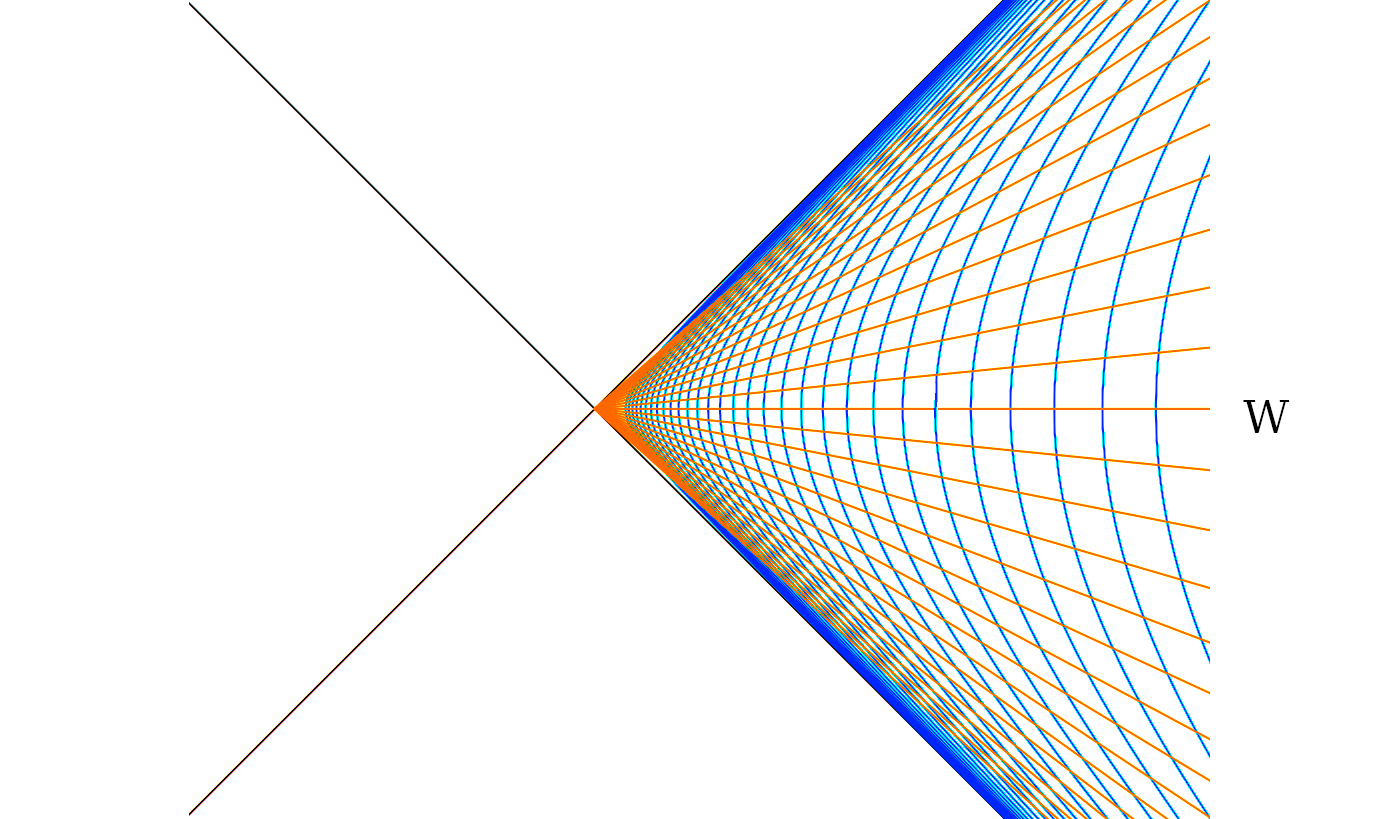
\includegraphics[scale=0.2]{rindler_w.png}
\caption{Rindler wedge I on the right.}
\label{rindlerw}
\end{figure}

The massless Klein-Gordon equation in Rindler coordinates is
\begin{equation}
  \Box \phi = e^{-2a \xi}(-\partial_\eta^2 + \partial_\xi^2) \phi = 0
\end{equation}
The wave equation retains the same structure as the Minkowski case, up to the overall conformal factor $e^{-2a\xi}$. Since this factor does not affect the null structure of the equation, the mode solutions retain the same plane wave form but in the Rindler coordinates
\begin{equation}
 r_k(\eta,\xi) = \frac{1}{\sqrt{4 \pi \omega_k}} e^{-i(\omega_k \eta -k \xi)} + \text{h.c.}
\end{equation}
for each wave number $k$ and positive frequency $\omega_k = |k| > 0$.  These ``Rindler modes'' are in terms of $\eta$ and $\xi$ and are thus confined to the Rindler wedge $W$.  Since Rindler coordinates only cover region I (the right wedge), these modes are not defined globally in Minkowski space.

\subsection{Unruh Modes}
To understand how a uniformly accelerated observer perceives the Minkowski vacuum as a thermal bath, we construct the Unruh modes, analytic combinations of Rindler modes that correspond to positive-frequency solutions with respect to Minkowski time.

From now on let $\omega_k = k > 0$. Bogoliubov coefficients satisfy $\alpha_k^2 - \beta_k^2 = 1$, ensuring normalization. The expressions below reflect their standard form and the associated thermal weighting:
\begin{equation}
  \begin{aligned}
    \alpha_k &= \frac{e^{\frac{\pi\omega_k}{2a}}}{\sqrt{2 \sinh \frac{\pi \omega_k}{a}}} = \sqrt{\frac{1}{1 - e^{-2\pi\omega_k / a}}}  \\
    \beta_k &= \frac{e^{\frac{-\pi\omega_k}{2a}}}{\sqrt{2 \sinh \frac{\pi \omega_k}{a}}} = \sqrt{\frac{1}{e^{2\pi\omega_k / a} - 1}} \quad \text{(thermal form)} \\
  \end{aligned}
  \label{alpha_beta}
\end{equation}

We analytically continue\footnote{From the definitions and properties of $\sinh$ and $\cosh$, it follows that $a(\mp t + x) = e^{a(\pm \eta + \xi)}$.} the Rindler modes $r_k$ and $r_{-k}$ into the $(t,x)$ plane, with $i \epsilon$ prescription, to understand their frequency content with respect to Minkowski time. This continuation reveals a change in frequency character (positive to negative) across the branch cut\footnote{Specifically $r_{\pm k} = e^{\pm \frac{i \omega_k}{a}\log a(\mp t + x \pm i\epsilon)}$.}
\begin{equation}
  \begin{aligned}
    r_{+k} &= \frac{1}{\sqrt{4 \pi \omega_k}} e^{-i(\omega_k \eta - k \xi)} = \frac{1}{\sqrt{4 \pi \omega_k}} (a(-t + x + i \epsilon))^{\frac{i \omega_k}{a}} \\
    r_{-k} &= \frac{1}{\sqrt{4 \pi \omega_k}} e^{-i(\omega_k \eta + k \xi)} = \frac{1}{\sqrt{4 \pi \omega_k}} (a( t + x - i \epsilon))^{\frac{-i \omega_k}{a}} \\
  \end{aligned}
\end{equation}
Although $r_k$ and $r_{-k}$ are positive-frequency modes with respect to Rindler time $\eta$, analytic continuation across the branch cut into the left wedge reveals that they acquire negative-frequency components with respect to Minkowski time $t$; see the middle column in Figure \ref{unruh_rainbow}.

We recall the standard Minkowski positive-frequency plane wave modes, here with $k>0$:
\begin{equation}
  \begin{aligned}
    \varphi_{+k} &= \frac{1}{\sqrt{4 \pi \omega_k}} e^{-i(\omega_k t - k x)}\\
    \varphi_{-k} &= \frac{1}{\sqrt{4 \pi \omega_k}} e^{-i(\omega_k t + k x)}\\
  \end{aligned}
\end{equation}
We next construct the Unruh modes
\begin{equation}
  \begin{aligned}
    \mu^R_k &= \alpha_k r_{+k} + \beta_k \widetilde{r_{-k}^*} = \alpha_k r_{+k} - \beta_k l_{-k} \\
    &= \frac{1}{\sqrt{4 \pi \omega_k}\sqrt{2 \sinh \frac{\pi \omega_k}{a}}} \left( e^{\frac{\pi \omega_k}{2a}} \left(a(-t+x+i\epsilon)\right)^{\frac{i\omega_k}{a}} + e^{\frac{-\pi \omega_k}{2a}} \left(a(t+x-i\epsilon)\right)^{\frac{i\omega_k}{a}} \right) \\
    \mu^L_k &= \beta_k \widetilde{r_{+k}^*} + \alpha_k r_{-k}  = -\beta_k l_{+k} + \alpha_k r_{-k} \\
    &=\frac{1}{\sqrt{4 \pi \omega_k}\sqrt{2 \sinh \frac{\pi \omega_k}{a}}} \left( e^{\frac{-\pi \omega_k}{2a}} \left(a(-t+x+i\epsilon)\right)^{\frac{-i\omega_k}{a}} + e^{\frac{\pi \omega_k}{2a}} \left(a(t+x-i\epsilon)\right)^{\frac{-i\omega_k}{a}} \right) \\
  \end{aligned}
  \label{unruh_mode_def}
\end{equation}
Here, the tilde denotes opposite analytic continuation across the logarithmic branch cut, corresponding to the conjugate $i \epsilon$ prescription. Operationally, this captures the mode's behavior in the left wedge and is often written using left Rindler modes $l_k$ and $l_{-k}$, which have opposite sign and live in coordinates related by $t \to -t$, $x \to -x$ .

The functions $\mu^R_k$ and $\mu^L_k$ are analytic in the lower-half complex $t$-plane and decay at infinity, so they qualify as positive-frequency Minkowski modes. They form an alternative orthonormal basis of solutions to the Klein-Gordon equation, distinct from the plane waves $\varphi_{\pm k}$. The Unruh modes diagonalize the Minkowski vacuum in terms of Rindler particle states and thus provide the natural framework for describing the Unruh effect and the thermal response perceived by uniformly accelerated observers.

\begin{figure}[h]
\centering
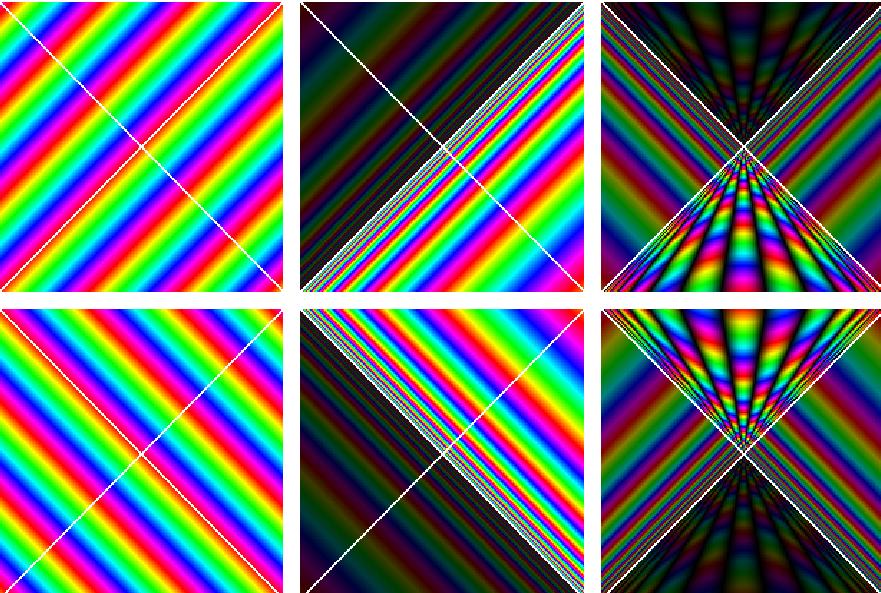
\includegraphics[scale=0.5]{unruh_mode_rainbow.png}
\captionsetup{width=0.7\textwidth}
\caption{Spacetime diagrams of the $k>0$ mode functions $\left[\begin{array}{ccc} \varphi_k & r_k & \mu^R_k \\ \varphi_{-k} & r_{-k} & \mu^L_k \end{array} \right]$. Color encodes the phase; brightness indicates magnitude. The Minkowski modes $\varphi_k$ and Unruh modes $\mu_k$ display consistent {\it rainbow} phase structure at $t=0$, reflecting their global positive-frequency character. In contrast, the Rindler modes $r_k$ flip phase across the horizon due to the analytic structure of the logarithm. The left-moving mode $r_k$ corresponds to emission; the right-moving $r_{-k}$ to absorption.}
\label{unruh_rainbow}
\end{figure}

\subsection{Bogoliubov Transforms}
We generalize the wedge $W$ to a translated wedge $W_c$ with apex $(0,c)$
\begin{equation}
 W_c = \{(t,x) : x - c > |t|\} 
\end{equation}
and a reflected (left) wedge $\widetilde{W}_c$ with apex $(0,c)$
\begin{equation}
 \widetilde{W}_c = \{(t,x) : x - c < -|t|\}.
\end{equation}
Let the superscripts $(0)$, $(c)$, $(\widetilde{c})$, and $(M)$ represent the $W_0$, $W_c$, $\widetilde{W}_c$, and Minkowski frames of reference respectively.  Let $(A \rightarrow B)$ represent an open set inclusion $A \subseteq B$.

In the Haag-Kastler framework of algebraic quantum field theory, the assignment of von Neumann algebras to spacetime regions defines a covariant functor: the inclusion of regions $A \rightarrow B$ induces an inclusion of algebras $\mathcal{A}(A) \rightarrow \mathcal{A}(B)$. Conversely, the Bogoliubov transformation given by $\alpha^{(A \rightarrow B)}$ and $\beta^{(A \rightarrow B)}$ defines a contravariant functor, acting on algebras via pullback. 

Since the analytically extended Rindler modes remain solutions of the Klein–Gordon equation, their inner products are preserved under continuation from the wedge to Minkowski space.  This allows us to directly compute $W_0 \rightarrow M$ Bogoliubov coefficients from equation (\ref{unruh_mode_def})
\begin{equation}
  \left[ \begin{array}{l}
    a^{(0)}_k \\
    a^{(0)}_{-k} \\
    \hline
    a^{(0)\dagger}_k \\
    a^{(0)\dagger}_{-k} \\
 \end{array} \right] = 
  \left[
\begin{array}{rr|rr}
    \alpha_k &       0   &  0       & \beta_k \\
    0        & \alpha_k & \beta_k & 0 \\
    \hline
    0        & \beta_k   & \alpha_k & 0 \\
    \beta_k &    0      &   0      & \alpha_k \\
\end{array} \right]_{k,q}
\left[ \begin{array}{l}
    c^R_q \\
    c^L_q \\
    \hline
    c^{R\dagger}_q \\
    c^{L\dagger}_q \\
 \end{array} \right]
\end{equation}
for a change of basis from $a^{(M)}_q$ to $c^R_q$ and $c^L_q$
\begin{equation}
  \phi = \int \dv{q} \mu_q^R c_q^R + \mu_q^L c_q^L + \text{h.c.}
  \label{c_ladder}
\end{equation}
So that we can summarize the transform as
\begin{equation}
  a_k^{(0)} = \alpha_k c_q^R + \beta_k c_q^{L\dagger}
\label{a_in_c}
\end{equation}

We next compute the more general mixed Bogoliubov transformations.
\begin{equation}
  \begin{array}{rll}
  (c \rightarrow M) : & a^{(c)}_k &= \int \dv{q} \alpha^{(c \rightarrow M)}_{kq} a^{M}_q + \beta^{(c \rightarrow M)}_{kq} a^{(M)\dagger}_q \\
  (c \rightarrow 0) : &   a^{(c)}_k &= \int \dv{q} \alpha^{(c \rightarrow 0)}_{kq} a^{(0)}_q + \beta^{(c \rightarrow 0)}_{kq} a^{(0)\dagger}_q \\
  (\widetilde{c} \rightarrow 0) : &   a^{(\tilde{c})}_k &= \int \dv{q} \alpha^{(\widetilde{c} \rightarrow 0)}_{kq} a^{(0)}_q + \beta^{(\widetilde{c} \rightarrow 0)}_{kq} a^{(0)\dagger}_q \\
  \end{array}
\end{equation}
We make use of a gamma function for $(c \rightarrow M)$. This occurs naturally in the KG dot product as an integral over an exponential phase from $\varphi_k$, and a $(x-c)$ power from $r_k^{(c)}$:
\begin{equation}
  \begin{array}{ccl}
    \alpha^{(c \rightarrow M)}_{kq} &= \left<\varphi_q, r_k^{(c)} \right> &= \frac{1}{a \pi} \sqrt{\frac{\omega_k}{\omega_q}} \left(\frac{a}{q}\right)^{\frac{i\omega_k}{a}} e^{\frac{\pi \omega_k}{a}} \Gamma\left(\frac{i\omega_k}{a}\right) \\
    \beta^{(c \rightarrow M)}_{kq} &= \left<\varphi_q^*, r_k^{(c)} \right> &= \frac{1}{a \pi} \sqrt{\frac{\omega_k}{\omega_q}} \left(\frac{a}{q}\right)^{\frac{-i\omega_k}{a}} e^{\frac{-\pi \omega_k}{a}} \Gamma\left(\frac{-i\omega_k}{a}\right) \\
  \end{array}
  \label{bogoCM}
\end{equation}
Next we consider products of shifted powers to go after $(c \rightarrow 0)$. We make use of a beta function for $(c \rightarrow 0)$ which occurs naturally in the KG dot product as an integral over a power of $x$ and of $x-c$, from $r_k^{(0)}$ and $r_k^{(c)}$ respectively.  We compute the Bogoliubov coefficients as
\begin{equation}
  \begin{aligned}
    \alpha^{(c \rightarrow 0)}_{kq} &= \left<r_q^{(0)}, r_k^{(c)} \right> = \frac{1}{2 \pi a}\sqrt{\frac{\omega_k}{\omega_q}} (ac)^{\frac{i(\omega_k - \omega_q)}{a}} B\left(\frac{i\omega_k}{a}, \frac{-i(\omega_k - \omega_q)}{a}\right) \\
    \beta^{(c \rightarrow 0)}_{kq} &= \left<r_q^{(0)*}, r_k^{(c)} \right> = \frac{1}{2 \pi a}\sqrt{\frac{\omega_k}{\omega_q}} (ac)^{\frac{i(\omega_k + \omega_q)}{a}} B\left(\frac{i\omega_k}{a}, \frac{-i(\omega_k + \omega_q)}{a}\right) \\
  \end{aligned}
  \label{bogoC0}
\end{equation}
The reflected diamond wedge version also yields a beta function, but with a different form
\begin{equation}
  \begin{aligned}
    \alpha^{(\widetilde{c} \rightarrow 0)}_{kq}     &= \left<r_q^{(0)*}, r_k^{(\widetilde{c})} \right> = \frac{1}{2 \pi a}\frac{\sqrt{\omega_k \omega_q}}{\omega_q - \omega_k} (ac)^{\frac{i(\omega_k - \omega_q)}{a}} B\left(\frac{i\omega_k}{a}, -\frac{i\omega_q}{a}\right) \\
    \beta^{(\widetilde{c} \rightarrow 0)}_{kq} &= \left<r_q^{(0)}, r_k^{(\widetilde{c})} \right> = \frac{1}{2 \pi a}\frac{\sqrt{\omega_k \omega_q}}{\omega_q + \omega_k} (ac)^{\frac{i(\omega_k + \omega_q)}{a}} B\left(\frac{i\omega_k}{a}, \frac{i\omega_q}{a}\right) \\
  \end{aligned}
  \label{bogoTC0}
\end{equation}


We can compare absolute magnitudes for $M$ v.s. $W_c$ and see that they don't depend on $q$ or $c$
\begin{equation}
  \begin{array}{cc}
    \left|\beta_{kq}^{(c_1 \rightarrow M)}\right|^2 = \left|\beta_{kq}^{(c_2 \rightarrow M)}\right|^2 & \\
    \left|\beta_{kq}^{(c_1 \rightarrow M)}\right|^2 = \left|\beta_{kq}^{(c_2 \rightarrow M)}\right|^2 & \\
 \end{array}
\end{equation}
The $c$ independence is expected since Unruh radiation is translation invariant. The $q$ independence can be strengthened as the expected number of particles in mode $k$
\begin{equation}
 \int \dv{q} \left|\beta_{kq}^{(c \rightarrow M)}\right|^2 = \frac{e^{\frac{-2 \pi \omega_k}{a}}}{2 \sinh \frac{\pi \omega_k}{a}} \int \dv{q} \frac{2}{a\pi |q|}
\end{equation}
where we factor out the divergent part to recover the radiation equation again\footnote{We frequently use here and elsewhere $|\Gamma(ib)|^2 = \frac{\pi}{b \sinh \pi b}$}.

We next turn to $(c \rightarrow 0)$ and also find $c$ independence there 
\begin{equation}
  \begin{array}{c}
    \left|\alpha_{kq}^{(c_1 \rightarrow 0)}\right| = \left|\alpha_{kq}^{(c_2 \rightarrow 0)}\right| \vspace{4pt} \\
    \left|\beta_{kq}^{(c_1 \rightarrow 0)}\right| = \left|\beta_{kq}^{(c_2 \rightarrow 0)}\right| \\
  \end{array}
\end{equation}
which is somewhat more surprising since this implies that $\int \dv{q} \left|\beta_{kq}^{(c_2 \rightarrow c_1)}\right|^2$ are $c_1$ and $c_2$ independent quantities for every shifted (and reflected resp.) wedge inclusion.

In other words, for shifted wedges\footnote{Similar statements are true for reflected (diamond) wedge inclusions}, the expected number of particles for a mode $r^{(c_2)}_k$ of $W_{c_2}$ in $W_{c_1}$'s vacuum is independent of the choice of shift $c_2$ and $c_1$. More explicitly we have a transform matrix of $\Lambda_c$ from $W_0$ to $W_c$ 
\begin{equation}
  \left[ \begin{array}{l}
    a^{(c)}_k \\
    a^{(c)}_{-k} \\
    \hline
    a^{(c)\dagger}_k \\
    a^{(c)\dagger}_{-k} \\
 \end{array} \right] = \underbrace{
  \left[
\begin{array}{rr|rr}
    A_c        &       0   &  B_c            &  0 \\
    0        &      -A_c   &  0            & -B_c \\
    \hline
    \overline{B_c}        &    0      &  \overline{A_c} & 0 \\
    0 &    -\overline{B_c}      &   0           & -\overline{A_c} \\
\end{array} \right]_{k,q} }_{\Lambda_c}
  \left[ \begin{array}{l}
    a^{(0)}_q \\
    a^{(0)}_{-q} \\
    \hline
    a^{(0)\dagger}_q \\
    a^{(0)\dagger}_{-q} \\
 \end{array} \right]
\end{equation}
where $A_c = \alpha_{kq}^{(c \rightarrow 0)} = P_c A_1 P_c^{-1}$  and $B_c = \beta_{kq}^{(c \rightarrow 0)} = P_c B_1 P_c$ for a diagonal phase factor matrix
\begin{equation}
  P_c = P_{c,rs} = \delta(r - s) c^{\frac{i\omega_r}{a}} = e^{\frac{i H}{a} \log c}
\end{equation}
We can write $\Lambda_c$ out compactly out as
\begin{equation}
  \Lambda_c = Q_c \Lambda_1 Q_c^{-1}
\end{equation}
where
\begin{equation}
  Q_c = \left[\begin{array}{cccc}
        P_c, & 0 & 0 & 0 \\
        0 & P_c & 0 & 0 \\
        0 & 0 & P_c^{-1} & 0 \\
        0 & 0 & 0 & P_c^{-1} \\
    \end{array} \right] 
\end{equation}
Note that $\lim_{c\to 0} \Lambda_c = 1$ since the limit of $\lim_{c\to 0} \alpha_{kq}^{(c \rightarrow 0)} = 1$ and $\lim_{c\to 0} \beta_{kq}^{(c \rightarrow 0)} = 0$, which corresponds nicely to $\lim_{c\to 0} W_c = W_0$. The composition of Bogoliubov transforms, $\Lambda_{nc} = \Lambda_c^n$, yields
\begin{equation}
  \begin{array}{ll}    
    Q_{nc} \Lambda_1 Q_{nc}^{-1}  &= \Lambda_{nc} \\
         &= \left(Q_c \Lambda_{c} Q_c\right) \left( Q_c^{-1} \Lambda_{c} Q_c\right) \cdots \left(Q_c \Lambda_{c} Q_c\right) \\
  &= Q_c \Lambda_c^n Q_c^{-1} \\
  \end{array}
\end{equation}
so that
\begin{equation}
  \begin{array}{ll}
  \Lambda_c^n &= Q_c^{-1} Q_{nc} \Lambda_1 Q_{nc}^{-1} Q{c} \\
  &= Q_n \Lambda_1 Q_n^{-1}
  \end{array}
\end{equation}
and more generally we have a one parameter group given by
\begin{equation}
  \left\{\Lambda_0^x = Q_x \Lambda_0 Q_x^{-1} : x \in \mathbb{R} \right\}.
\end{equation}
These Bogoliubov transformations between shifted wedges define a one-parameter group, reflecting an underlying symmetry structure. This naturally connects to modular flow as studied in algebraic QFT, where such transformations correspond to automorphisms generated by the modular operator. This is an explicit realization of modular flow, due to the von Neumann algebra modular automorphism associated with the translation $W_0 \rightarrow W_c$, studied in detail in Tomita-Takesaki theory \cite{Borchers2000}.  There we find thermal KMS states between open set inclusions in a much more general setting.


Consider a sequence
\begin{equation}
  W_{c_n} \subseteq \cdots \subseteq W_{c_i} \subseteq \cdots \subseteq W_{c_j} \subseteq W_{c_2} \subseteq W_{c_1}
\end{equation}
Then each $W_{c_i} \subseteq W_{c_j}$ involves particle production with a fixed squared magnitude for mode $k$.  We calculate this expected number of $W_{c_i}$ particles for mode $k$ in $W_{c_j}$'s vacuum
\begin{equation}
  \bra{0_{W_{c_j}}} a^{(c_i)\dagger}_k a^{(c_i)}_k \ket{0_{W_{c_j}}} = \frac{1}{2 \pi^2 k \sinh \frac{\pi k}{a}} \int_{x=0}^\infty \frac{x \sinh x}{(x+\frac{\pi k}{a}) \sinh(x+\frac{\pi k}{a})}
\end{equation}
which diverges.  The integrand goes to $e^{-\frac{\pi k}{a}}$ as $x$ gets large, so we can see that the expected number of particles in ratio goes to another thermal form
\begin{equation}
  \frac{1}{m (e^{2m} + 1)} = \frac{1}{k (e^{\frac{2\pi \omega_k}{a}} - 1)}.
\end{equation}

\section{Driving Sources}

We now ask a fundamental question: {\bf ``What exactly is accelerating the observer?''} Until this point, we've treated acceleration as a coordinate choice, without invoking any underlying physical mechanism. We have also not specified the observer’s precise location within the Rindler wedge, nor the spatial origin of the observed excitations. These ambiguities reflect the effective coarse-graining over the observer's details, a feature that contributes to the thermal character of the Unruh effect.

Figure \ref{emit_absorb} illustrates the situation for a sharply peaked frequency wave packet made of Rindler modes. The modes $r_k$ are left-moving, propagating toward the future horizon and are interpreted as {\bf emission}. The $r_{-k}$ modes are right-moving, originating from the past horizon and are interpreted as {\bf absorption}. The Rindler modes are constructed as superpositions of Minkowski modes \(\varphi_q\), effectively smeared over a range of frequencies. This is visually evident in Figure \ref{unruh_rainbow}, where the local frequencies increase (blue-shift) near the horizons. This is made explicitly by the Bogoliubov coefficients \(\alpha_{kq}^{(c \rightarrow M)}\) and \(\beta_{kq}^{(c \rightarrow M)}\) which encode the Fourier decomposition of the Rindler modes through their Klein-Gordon inner products with the Minkowski modes \(\varphi_q\) and \(\varphi_q^*\), respectively. This frequency delocalization, tied to the observer's acceleration horizon, underlies the apparent thermal character of the radiation.

\begin{figure}[h]
\centering
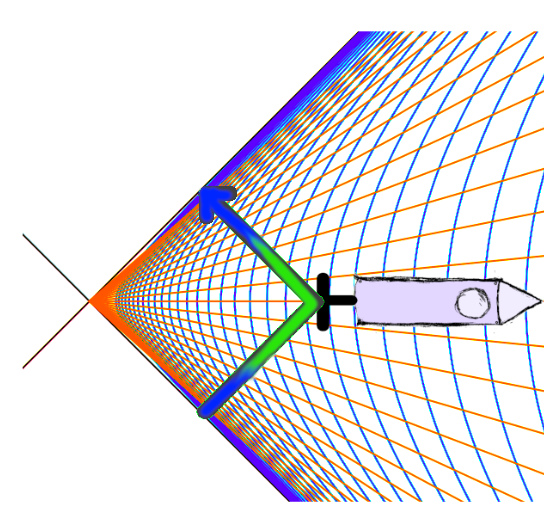
\includegraphics[scale=1.5]{emit_absorb.png}
\captionsetup{width=0.7\textwidth}
\caption{
  A Rindler mode's frequency is smeared out in Minkowski space, blue-shifted near the horizon. We diagram a particle as if it were striking a mirror at the rear of a rocket, where its reflection emerges as a combination of emission and absorption processes in the Rindler frame.}
\label{emit_absorb}
\end{figure}

To address this, we introduce a driving source, a physical mechanism responsible for the field's excitation and, indirectly, for the observer's acceleration. This reframes the interpretation: the radiation is not spontaneous but instead emerges as a coherent response to the source, see illustration in Figure \ref{rocket_inertial}. The apparent thermality, then, is tied to our ignorance of the source's detailed structure.

We aim to encode the effect of a creation operator by introducing a source term $J(x)$ into the Lagrangian at some distant time in the past, which directly excites the field in a specific mode. Since $J(x)$ couples linearly, it prepares a coherent state that excites the chosen mode in a controlled, phase-coherent manner. To replicate the action of a creation operator, the source must be engineered such that its overlap with the mode functions $u_k(x)$ matches the operator’s action on the field.

\begin{figure}[h]
\centering
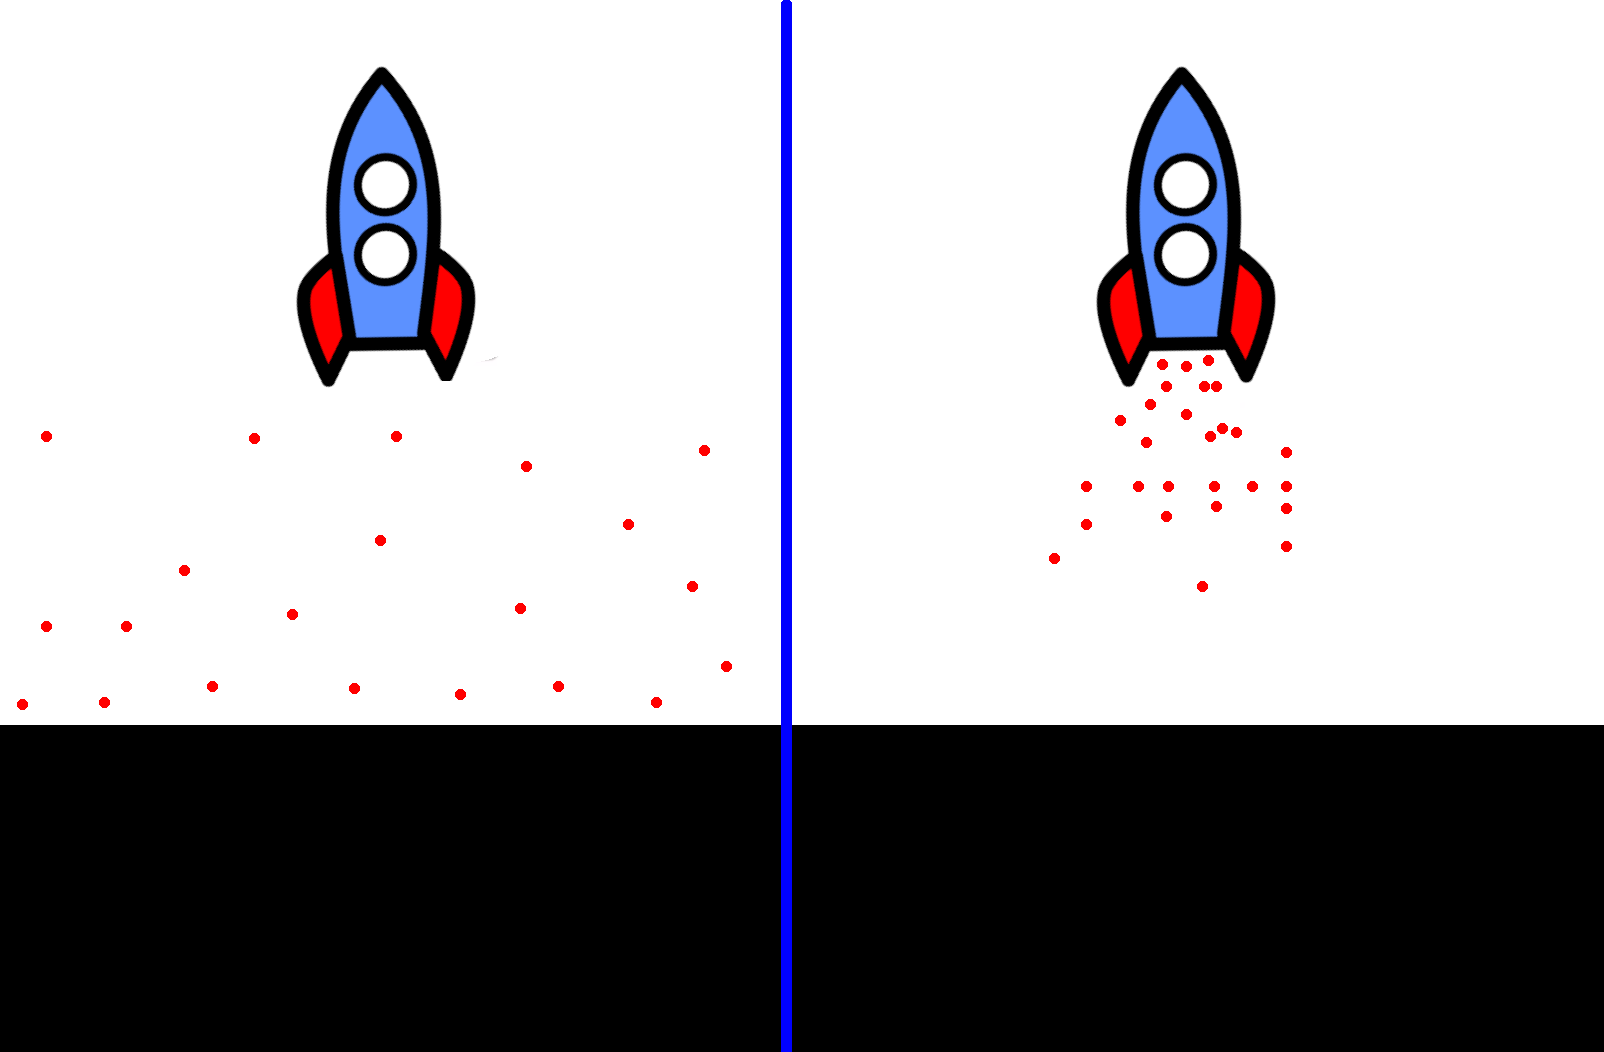
\includegraphics[scale=0.5]{rocket_inertial.png}
\caption{Conceptual illustration of thermal v.s. localized acceleration.}
\label{rocket_inertial}
\end{figure}

The field can be expanded as in equation (\ref{c_ladder}), and the $\beta_k$-term in equation (\ref{a_in_c}) is responsible for the thermal particle content of the Minkowski vacuum as seen by Rindler observers. For clarity, we first present the construction for a single positive-frequency $\mu^{L*}_k$-mode. Because the Unruh modes form a complete orthonormal set under the Klein-Gordon inner product, this construction extends linearly and independently to the full family of modes. We encode the effect of a creation operator $c_k^{L \dagger}$ using
\begin{equation}
  c _k^{L\dagger} = \left<\phi, \mu_k^{L*}\right>_{KG} = \int \dv{x} \mu_k^{L*}(x) \phi(x)
\end{equation}
and the orthogonality of the mode functions in the Klein-Gordon inner product.

Although the Unruh modes involve both left- and right-moving Rindler components, associated with emission and absorption in the accelerated frame, they are constructed to have purely negative frequency with respect to Minkowski time. This ensures that the source couples to physical creation operators and injects particles into the field in a well-defined way. The resulting excitation respects the correct Minkowski vacuum structure while encoding the full Rindler response.

In the generating functional formalism, setting $J_k^L(x) = -\beta_k u_k^{L*}$ the functional derivative $\frac{\delta}{\delta J_k^L}Z[J_k^L]|_{J_k^L=0}$ inserts $\phi$ into time-ordered correlators. Smearing this field insertion against $\mu_k^{L*}(x)$ thus projects onto $c_k^{L\dagger}$ and we have\footnote{The remaining $\alpha_k$ factor reflects the mismatch between the squeezed Unruh vacuum and the coherent state prepared by the source.}
\begin{equation}
\begin{array}{ll}
  a_k^{(0)J} &= \alpha_k c_q^R + \beta_k c_q^{L\dagger} -  \beta_k c_q^{L\dagger} \\
  &= \alpha_k c_q^R
\end{array}
\end{equation}

In Rindler coordinates, this source term prepares a modified field state in which the Rindler mode occupation differs from the thermal distribution of the Minkowski vacuum. Rather than simply adding energy, the source introduces a coherent excitation that cancels the mode structure induced by the Bogoliubov $\beta$-terms, effectively replacing their contribution. This lets us construct a state where the Rindler response is vacuum-like for mode k

\begin{equation}
  \bra{J_k^L}  b_k^{\dagger} b_k \ket{J_k^L} = \bra{0_M}  b_k^{J_k^L \dagger} b^{J_k^L}_k \ket{0_M} = 0
\end{equation}

As a result, the source reproduces the exact Rindler particle spectrum predicted by the Rindler–Minkowski Bogoliubov transformation, provided the excited modes are drawn from a Klein-Gordon orthonormal basis such as the Unruh modes; this holds when using causal (retarded) or time-ordered (Feynman) Green’s functions, both of which allow linear superpositions of negative-frequency modes to generate particle injection.

\section{Subwedge Localization in Rindler Space}
\subsection{Localization via Translated Wedge Inclusion}

Consider the two nested Rindler wedges $W_c \subseteq W_0$ as shown in Figure \ref{restrict}. Let $r_q$ denote a Rindler mode associated with $W_0$, analytically continued to the entire Minkowski space. The gray-scale region indicates the full support of $r_q$, while the rainbow-colored segment shows its restriction to the smaller wedge $W_c$.

\begin{figure}[h]
  \centering
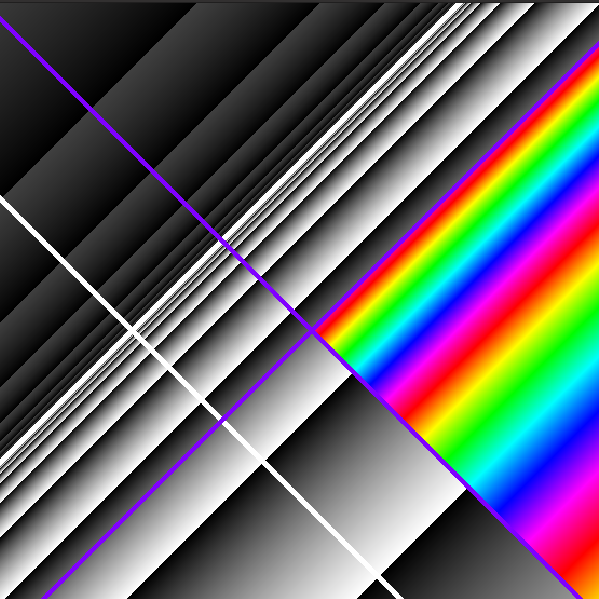
\includegraphics[scale=0.4]{wedge_in_wedge.png}
\caption{A Wedge $W_c$ (blue) inside of the wedge $W_0$ (white). Rindler mode $r_q$ of $W_0$ (gray-scale) restricted to $W_c$ (rainbow).}
\label{restrict}
\end{figure}

By considering the restriction of $r_q$ to $W_c$, we have partially localized the observer and the mode. The restriction effectively cuts off the high-frequency content of $r_q$ near the future horizon\footnote{Similarly, $r_{-q}$ experiences suppression near the past horizon.}. The resulting mode still spans the full spatial extent of $W_c$, but it is now insulated from the highly oscillatory behavior near the horizons of $W_0$.  The localization is not complete however, the observer can still be anywhere within the wedge $W_c$, and the corresponding modes $r_k$ still exhibit thermal characteristics because of low-frequency oscillations extending throughout the wedge.

To further study the situation, consider the modulus squared inner product $\left|\left<r_q^{(0)}, r_k^{(c)} \right>\right|^2$, also known as the Bogoliubov $\left|\alpha^{(c \rightarrow 0)}_{kq}\right|$, from equation (\ref{bogoC0}).  We fix $q$ and view
\begin{equation}
  \left|\left<r_q^{(0)}, r_k^{(c)} \right>\right|^2 = \frac{\sinh \frac{\pi \omega_q}{a}}{4\pi a (\omega_q - \omega_k) \sinh \frac{\omega_q - \omega_k}{a} \sinh \frac{\pi \omega_k}{a}}
\end{equation}
as a function of $\omega_k$. The function exhibits a second-order pole at $\omega_k = \omega_q$, resulting in a sharply peaked spectral response, see Figure $\ref{peaked}$. The thermal character is evident in the $\sinh$ terms: $\sinh \frac{\pi \omega_k}{a}$ introduces a broadening near $\omega_k = 0$, while $(\omega_q - \omega_k) \sinh \frac{\omega_q - \omega_k}{a}$ contributes thermal spreading near the peak at $\omega_k = \omega_q$. However, the pronounced spectral peak at $\omega_k = \omega_q$ arises not from thermal effects but from the localization itself.

\begin{figure}[h]
  \centering
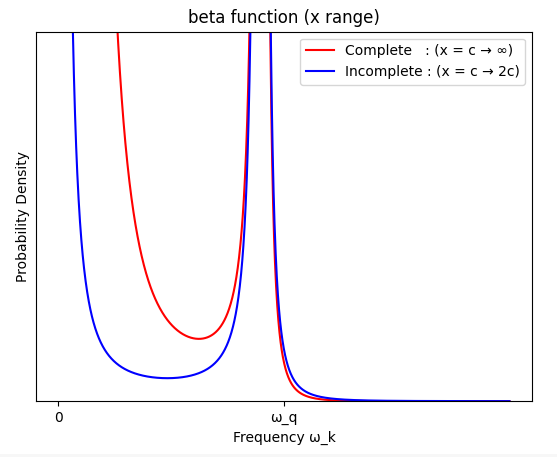
\includegraphics[scale=0.6]{peaked.png}
\caption{The Rindler modes $r_k$ of $W_c$ show a peaked spectral overlap with $r_q$ at $\omega_k = \omega_q$. The incomplete beta function picks out the spectral peak supressing the peak at zero.}
\label{peaked}
\end{figure}

\subsection{Diamond Localization via Reflected Wedge Intersection}

Further localization is achieved by intersecting $W_c$ with a reflected wedge $\widetilde{W}_{2c}$, where the reflection is taken about the origin. This defines a more tightly localized diamond-shaped region, as shown in Figure \ref{diamond}. The mode $r_q$ is now restricted to the intersection $W_c \cap \widetilde{W}_{2c}$, which eliminates much of the infrared divergence previously associated with the unrestricted wedge.

The inner product now takes the form of an incomplete version of the beta function from equation (\ref{bogoC0}), corresponding to an integral evaluated from $c$ to $2c$ rather than extending to infinity. The resulting spectral response, computed from this truncated integral, is shown in Figure \ref{peaked}. The plot reveals that the main spectral peak at $\omega_k = \omega_q$ persists, while the thermal contribution near $\omega = 0$ is significantly attenuated.

Rather than viewing $r_q$ as an element in a Bogoliubov transformation between full mode bases, we can instead interpret it as a driving source defined originally over the wedge $W_0$. The restriction to $W_c$ then acts to filter this source, removing its high-frequency behavior near the horizon, while the further restriction to the diamond $W_c \cap \widetilde{W}_{2c}$ suppresses long-wavelength contributions that would extend outside the compact region. In this sense, the diamond does not host a new mode basis per se, but serves as a localized detection region for the filtered signal. The observed spectral response in the diamond thus reflects the interplay between the support of the original source and the geometric constraints imposed by the intersection. This perspective shifts the emphasis from complete mode decompositions to causal influence and spectral imprint within a localized domain.

\begin{figure}[h]
  \centering
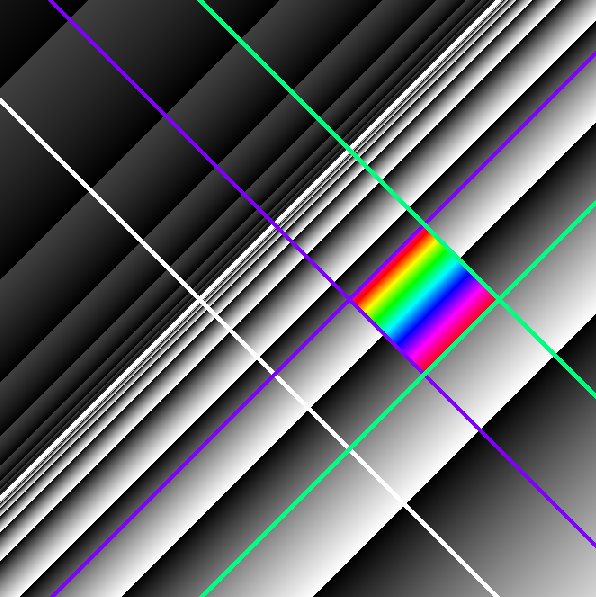
\includegraphics[scale=0.4]{diamond_in_wedge.png}
\caption{The same situation as in Figure \ref{restrict} but we further intersect with a reflected (left) wedge $\widetilde{W}_{2c}$ (green). Rindler mode $r_q$ of $W_0$ (gray-scale) restricted to $W_c \cap \widetilde{W}_{2c}$ (rainbow).}
\label{diamond}
\end{figure}




\subsection{Wave Packet Interpolation}
Let $N = e^{-\frac{1}{2} \frac{(x-t-\mu)^2}{\sigma^2}}$ then using the Parabolic cylindrical function\footnote{$\int_{t=0}^\infty e^{-zt} t^{a-\frac{1}{2}} e^{-\frac{1}{2} t^2} \dv{t} = e^{\frac{1}{4}z^2} \Gamma\left(a + \frac{1}{2}\right) D_{-a - \frac{1}{2}}\left(z\right)$, and $U(a,z) = D_{-a - \frac{1}{2}}\left(z\right)$} $D_\nu(z)$ we have

\begin{equation}
  \left< \varphi_q N, r_k \right> = \frac{1}{2\pi a} \sqrt{\frac{\omega_k}{\omega_q}} (\sigma a)^\frac{i\omega_k}{a} e^{-\frac{1}{4}\left(i q \sigma - \frac{\mu}{\sigma}\right)^2} e^{-\frac{1}{2} i q} \Gamma\left(\frac{i \omega_k}{a}\right) D_{-\frac{i\omega_k}{a}}\left(iq\sigma - \frac{\mu}{\sigma}\right)
\end{equation}
and then
\begin{equation}
  \left|\left< \varphi_q N, r_k \right>\right|^2 = \frac{1}{4a\omega_q} e^{-\frac{1}{2} \left(\frac{\mu^2}{\sigma^2} - a^2 \sigma^2\right)} \frac{\left| D_{-\frac{i\omega_k}{a}}\left(iq\sigma - \frac{\mu}{\sigma}\right) \right|^2}{\sinh \frac{\pi \omega_k}{a}}
\end{equation}
From \cite{Olver1959UniformAE} we have
\begin{equation}
  U(a, -z) = e^{-i\pi(a + \frac{1}{2})}z^{-a - \frac{1}{2}}e^{-\frac{1}{4}z^2} \{ 1 + O(|z|^{-2}) \} + \frac{(2 \pi)^{\frac{1}{2}}}{\Gamma(\frac{1}{2} + a)} z^{a-\frac{1}{2}} e^{\frac{1}{4}z^2} \{1 + O(|z|^{-2})\}
\end{equation}
when $-\frac{3}{4}\pi + \epsilon \le \arg z \le \frac{1}{4} \pi - \epsilon$.

\section{Conclusion and Prediction}

This work reframes the Unruh effect as a localized, mechanistic response to directed energy input, thrust, rather than as a consequence of horizon thermality. By restricting Rindler modes to subwedges and their intersections via modular automorphisms, we show that the apparent thermal behavior arises from nonlocal mode mixing, not fundamental statistics. Using parabolic cylinder functions, we construct smooth, localized wave packets that interpolate between global and compact support, revealing how detector response depends on localization scale. While our results focus on flat spacetime, the framework naturally suggests a path forward: the same techniques may shed light on Hawking radiation by modeling localized excitations near black hole horizons. This possibility is illustrated in Figure \ref{rocket}, which shows how similar localization might be applied.

\begin{figure}[h]
\centering
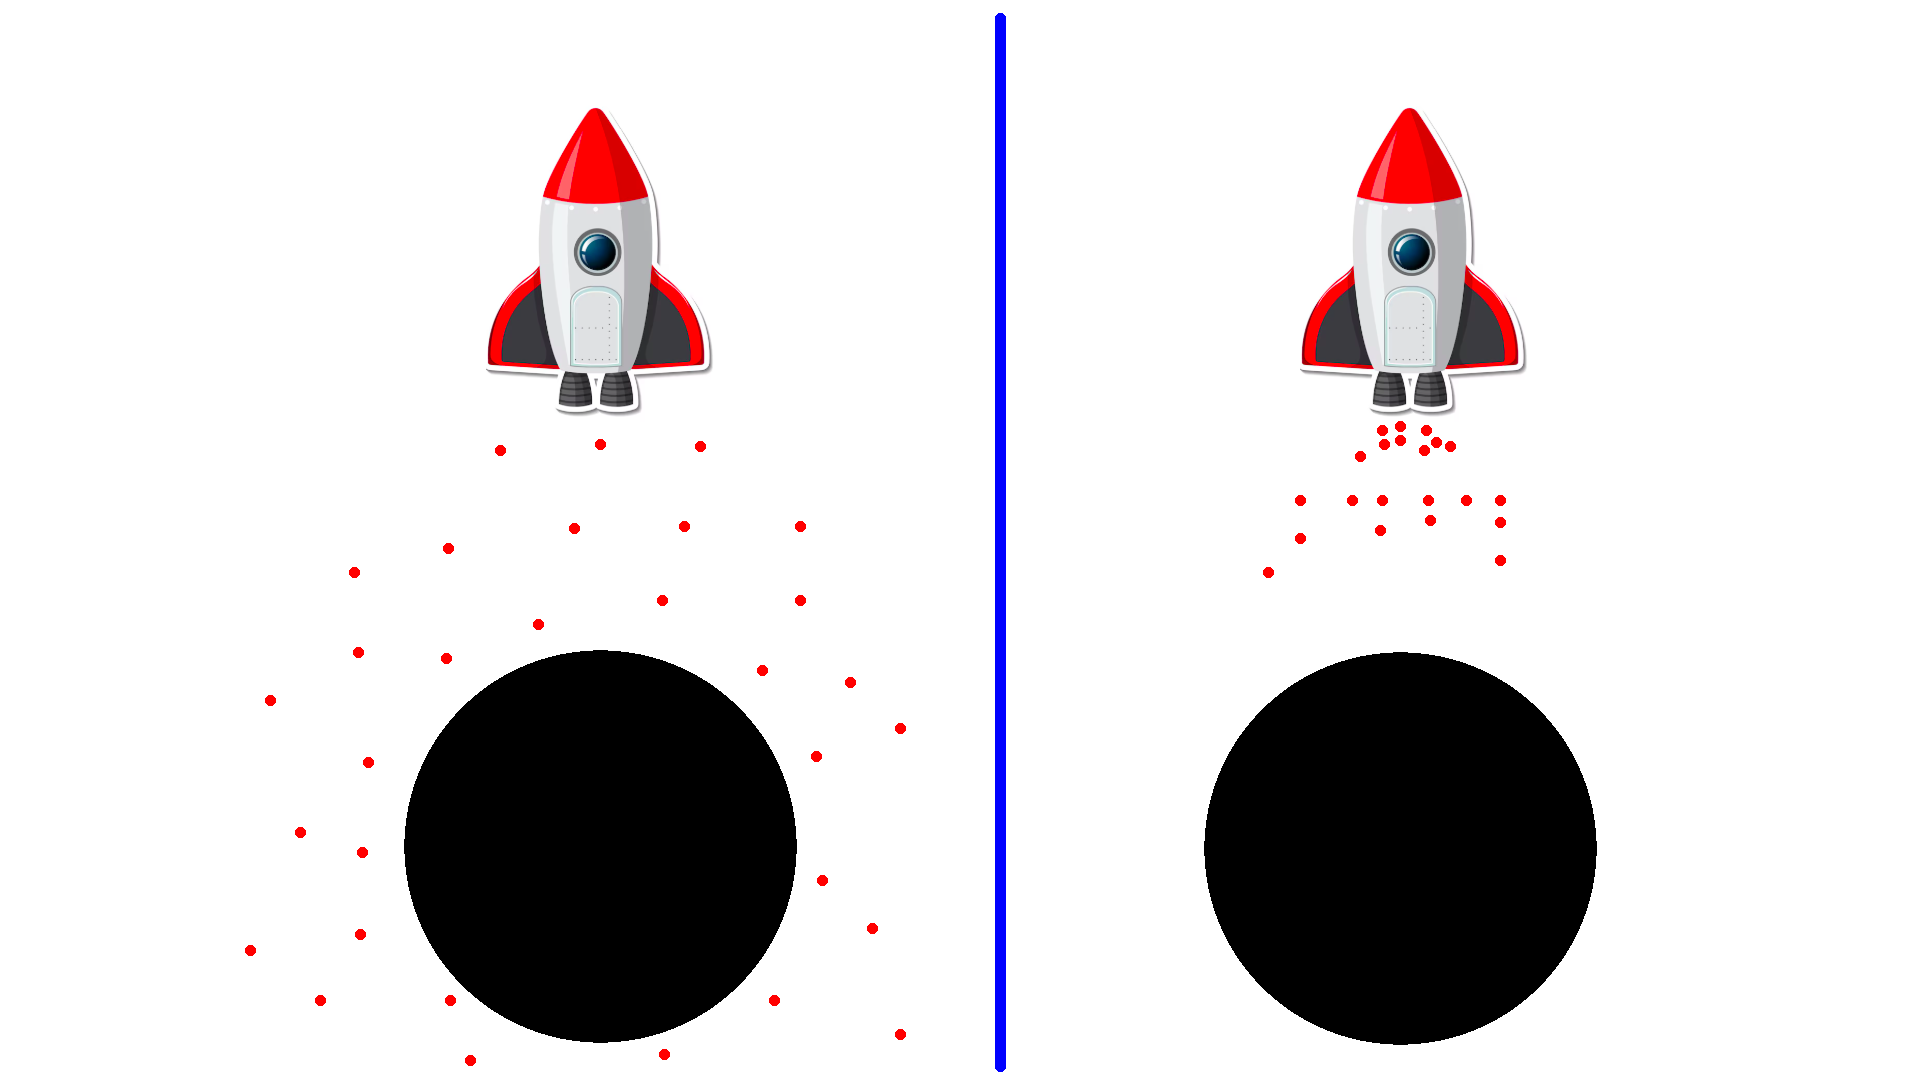
\includegraphics[scale=0.5]{rocket.png}
\caption{Hawking picture of black hole radiating on the left. Our picture of a rocket thrusting on the right.}
\label{rocket}
\end{figure}

\section{Acknowledgments}
Thanks to Ben Commeau and Daniel Justice for useful discussions.

\section{Notes}
To go after $(c \rightarrow M)$ we start with a useful formula obtained by taming Fourier oscillations and doing contour integrals
\begin{equation}
  \int_{-\infty}^\infty e^{ikx} (x \pm i \epsilon) ^b \dv{x} = -\frac{2i}{k^{b+1}} e^{\frac{-\pi b}{2}} \Gamma(b+1)
\end{equation}

\begin{equation}
  \int_{c}^\infty x^a (x-c)^b \dv{x} = c^{a+b+1} B(b+1, -a-b-1)
\end{equation}
and over sign choices $b,d \in \{-1,1\}$
\begin{equation}
  f_{k,b,d} = \left(a\left(b(t-i\epsilon)+x\right)\right)^\frac{id\omega_k}{a}
\end{equation}
we have the dot product
\begin{equation}
  \left< f_{k,b_k,d_k}, f_{q,d_q,d_q}\right> = \frac{1}{2\pi} \sqrt{\frac{\omega_k}{\omega_q}} (ac)^\frac{i(d_k\omega_k - d_q \omega_q)}{a} \left((-d_k)\frac{b_k + b_q}{2} \right) B\left(\frac{id_k\omega_k}{a}, \frac{-i(d_k\omega_k - d_q \omega_q)}{a}\right)
\end{equation}



\bibliographystyle{ieeetr}
\bibliography{bibliography}

\end{document}
